\documentclass[10pt,twocolumn]{article}
\usepackage[margin=1.9cm,columnsep=0.55cm]{geometry}
\usepackage{amsmath,amssymb,graphicx,booktabs,microtype}
\usepackage[hidelinks]{hyperref}
\usepackage[small,compact]{titlesec}
\setlength{\parskip}{1pt}

\title{\vspace{-6mm}\large\bf Horizon-Gated JEPA: Label-Free Separation of\\
Slow and Fast Factors in Time Series}
\author{Jaechan Lee}
\date{July 24, 2026 --- two-page progress report}

\begin{document}
\maketitle
\vspace{-8mm}

\section{Motivation and hypothesis}
Practitioners want the \emph{slowly-varying state} of a time series ---
machine health, cardiac diagnosis, activity, regime --- but the observed
signal buries it under fast variation (per-revolution vibration, beat
morphology, sensor noise). Several important tasks need the two \emph{separated},
not merely both encoded: (a) \textbf{anomaly attribution} --- is an alarm a
point anomaly (instantaneous glitch) or a contextual one (slow drift away from
the current state)? the correct response differs; (b) \textbf{selective
robustness} --- a diagnosis that survives a change in the fast dynamics (new
sensor, new subject); (c) interpretation of a health trajectory. An entangled
embedding cannot provide these regardless of its accuracy.

Existing separators fall short in principle. Signal decomposition
(moving-average trend, wavelets, EMD) splits by \emph{frequency band}, but a
slow factor need not live in a low band --- in bearings the degradation state
is the \emph{envelope of high-frequency resonance} (why envelope analysis
exists), so a low-pass ``trend'' misses it. Sequential VAEs (DSAE, C-DSVAE)
separate a \emph{time-invariant} content code via reconstruction ELBOs ---
fragile under sensor noise and unable to represent factors that vary slowly
rather than never. Horizon-conditioned JEPAs (HEPA) internalize multi-scale
dynamics implicitly but do not factor them.

We use a purely functional criterion: \textbf{information useful for
predicting the far future is exactly the slow information}, and the prediction
horizon --- free in any predictive learner --- is the supervision. Our
hypothesis:

\emph{H1: in a horizon-conditioned JEPA, if the predictor's access to one
latent block is gated off for long horizons, slow factors concentrate in the
ungated block and fast factors are displaced to the gated block --- no labels.}

Two secondary hypotheses sharpen this. \emph{H2 (guarantee asymmetry):} the
gate structurally guarantees only \emph{inclusion} of slow information in the
ungated block; \emph{exclusion} of fast information relies on capacity
pressure and, if needed, a light decorrelation penalty. \emph{H3
(architecture specificity):} the gate should work on \emph{latent}-space
prediction but fail on raw-signal prediction, because raw targets force the
encoder to smear unpredictable detail across all dimensions.

\section{Method}
\textbf{Backbone (established).} We use a horizon-conditioned JEPA: a causal
encoder produces one embedding per patch; a predictor $P(z_t,\Delta)$ maps an
anchor embedding and a horizon $\Delta$ to a \emph{parallel, direct} prediction
of the target embedding at $t+\Delta$ (not autoregressive next-token). This is
the CPC multi-horizon predictor (van den Oord et al., 2018) with I-JEPA-style
EMA targets (Assran et al., 2023), as in HEPA (2026). \textbf{Our contribution}
is a gate on this backbone, not the backbone.
A causal encoder maps patches to embeddings
$z_t=[z^{\mathrm{slow}}_t;z^{\mathrm{fast}}_t]\in\mathbb R^{64}$ (slow block
deliberately narrow, 16 dims). The predictor, conditioned on
$\Delta\in\{1,4,16,64,128\}$ patches, regresses the EMA target encoder's
embedding at $t+\Delta$:
\[
\mathcal L=\textstyle\sum_{\Delta}\big\|
P\big(z^{\mathrm{slow}}_t,\;g(\Delta)\,z^{\mathrm{fast}}_t,\;\Delta\big)
- \bar z_{t+\Delta}\big\|^2
+\lambda\,\mathcal L_{\mathrm{dcor}},
\]
with a soft gate $g(\Delta)=\sigma\!\big((\tau-\Delta)/w\big)$: for
$\Delta\!\gg\!\tau$ the predictor sees only the slow block. The gate is
asymmetric by design --- short-horizon prediction keeps access to both blocks
because fast dynamics are \emph{conditioned on} slow state; blocking the slow
block at short horizons would force slow information to be duplicated into
the fast block. $\mathcal L_{\mathrm{dcor}}$ penalizes squared cross-covariance
between blocks (removes duplicates; cf.\ H2). The threshold is set from the
data itself as $\tau = c\,T_{\mathrm{ac}}$, where $T_{\mathrm{ac}}$ is the
signal's autocorrelation decay time (the lifetime of fast dynamics), $c\!\approx\!2.5$;
no sampling-rate knowledge is needed.

\section{Pilot setup}
\textbf{Data.} Synthetic series with recorded ground-truth factors: a slow
3-state Markov regime (mean dwell 3000 steps) setting carrier frequency
($\pm5\%$), and a fast OU process $u$ (lifetime 50 steps) that jitters the
instantaneous frequency by a comparable amount and adds a small direct term.
Amplitudes are identical across regimes, so \emph{no short-window statistic
reveals the regime}; identifying it requires integrating hundreds of steps.
Fast ground truth is $(u,\sin\varphi,\cos\varphi)$.
\textbf{Protocol.} Train on 1M steps; evaluate on a held-out 200k-step series.
Linear probes read each block; we report \emph{normalized information}:
probe score of a block divided by the full-embedding score (chance-corrected
for the regime). All variants share one backbone ($\sim$0.5M params), recipe,
and compute; $n{=}3$ seeds.
\textbf{Variants.} Ours (gate$+$dcor, $\lambda{=}4$); gate only; no gate
(= ungated horizon-JEPA, i.e.\ HEPA-style; its ``slow'' block is the same 16
indices, controlling for arbitrary splits); dcor only; and, for H3, an AR head
predicting raw future patches (next-token family) with and without the
identical gate.

\begin{figure}[t]
\centering
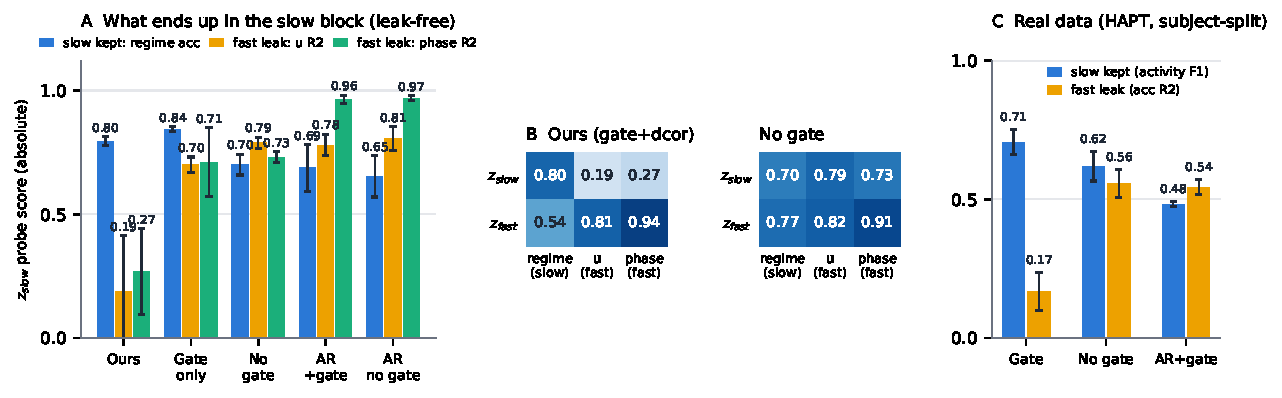
\includegraphics[width=\linewidth]{fig_main.pdf}
\vspace{-6mm}
\caption{\small \textbf{A:} fraction of the full embedding's information
retained in $z_{\mathrm{slow}}$ (3 seeds, $\pm$ sd). Ours keeps 98\% of the
slow factor while admitting only 22\%/15\% of the fast factors; without the
gate the slow block is a near-copy of everything (88\%/77\%); on raw-signal
prediction (AR) the identical gate separates nothing (rightmost pair).
\textbf{C:} the same contrast reproduced on real inertial data (HAPT).
\textbf{B:}
block$\times$factor matrices (ours vs.\ no gate).}
\vspace{-3mm}
\end{figure}

\section{Preliminary results}
\textbf{F1 --- the gate separates (H1).} With gate$+$dcor, $z_{\mathrm{slow}}$
(16 of 64 dims) retains $0.98$ of the full embedding's regime information
while fast-factor leakage drops to $0.22$ ($u$) and $0.15$ (phase), vs.\
$0.88/0.77$ for the ungated control --- a $4\times$ reduction, consistent
across seeds ($0.198\pm.023$ raw $R^2$). Reverse exclusion also emerges:
$z_{\mathrm{fast}}\!\to\!$regime drops $0.89\!\to\!0.73$.
\textbf{F2 --- latent targets are necessary (H3).} On raw-patch prediction
the identical gate moves fast leakage only from $0.95$ to $0.88$ ($u$) and
$0.99$ to $0.96$ (phase) --- essentially nothing, against $0.88\!\to\!0.22$
for latent prediction: horizon gating is specifically synergistic with the
JEPA family, not a generic trick. Contrastive methods (TS2Vec) admit no gate
at all --- their objectives contain no horizon variable.
\textbf{F3 --- structure assigns, penalty purifies (H2).} Gate alone reduces
leakage but incompletely ($0.68/0.61$); dcor alone \emph{degenerates} --- the
model satisfies decorrelation by emptying the slow block (regime probe
$0.53$, vs.\ $0.86$ full). Only the combination works: the gate gives each
block a job; the penalty removes duplicates.
\textbf{F4 --- tuning confirms the theory.} Sweeps: $\tau$ is best at
$\approx\!2.5\,T_{\mathrm{ac}}$ (worse at $0.6\times$ and $10\times$),
matching the intended placement between the fast lifetime and the slow dwell;
shrinking the slow block $16\!\to\!8$ dims cuts leakage to $0.11/0.00$ at
unchanged regime accuracy, directly evidencing the capacity-pressure
mechanism of H2; $\lambda{=}4$ balances purity vs.\ informativeness.
An earlier iteration also \emph{failed} informatively: when the fast factor's
lifetime was shorter than the shortest horizon, the gate had nothing to
separate --- the effect requires (and thus reflects) genuine multi-scale
structure in the data.
\textbf{F5 --- real data (Fig.~C, Tab.~1).} On two real datasets with a
genuine timescale gap the gate reproduces the synthetic separation ($n{=}3$
seeds). HAPT (smartphone inertial signals; slow = activity persisting
$\sim$12\,s, fast = gait, $T_{\mathrm{ac}}\!\sim\!0.1$\,s): the slow block's
activity information rises to $0.88$ of the full embedding (vs.\ $0.72$
ungated) while fast leakage drops $0.76\!\to\!0.31$. PTB-XL ECG (slow =
diagnosis, fast = beat morphology): a smaller but consistent effect (fast
leakage $0.66\!\to\!0.53$, or $0.40$ with dcor). On the AR head the gate does
nothing on both (H3). The decorrelation penalty \emph{hurts} on HAPT yet
\emph{helps} on PTB-XL --- its value is data-dependent, and the weaker PTB-XL
effect is expected since diagnostic cues partly live at the beat timescale,
blurring the slow/fast split. On XJTU-SY bearing vibration we
obtained two complementary results instead of a separation showcase:
(i) a low-pass baseline cannot recover the fault-carrying envelope
($R^2{=}{-}0.19$ vs.\ $0.65$ for the learned embedding) --- real-data
confirmation of the frequency$\neq$factor motivation; and (ii) measured
autocorrelation shows the accessible carrier and envelope proxies share
nearly the same timescale ($T_{\mathrm{ac}}\!\approx\!1$--$2$ patches), and
accordingly the gate does \emph{not} manufacture separation --- consistent
with F4: the method separates only where a genuine timescale gap exists.

\begin{table}[t]
\centering\small
\caption{\small Real-data separation (3 seeds). Slow-info = slow block's slow
factor score as a fraction of the full embedding (higher better); fast-leak =
slow block's fast-factor score, normalized (lower better).}
\begin{tabular}{@{}llcc@{}}
\toprule
Dataset & Variant & slow-info $\uparrow$ & fast-leak $\downarrow$ \\
\midrule
HAPT   & gate    & \textbf{0.91} & \textbf{0.31} \\
       & no gate & 0.78 & 0.76 \\
PTB-XL & gate+dcor & 0.97 & \textbf{0.40} \\
       & no gate & 0.96 & 0.66 \\
\bottomrule
\end{tabular}
\end{table}

\section{Planned work and limitations}
The clearest payoff of separation is \textbf{anomaly attribution}: reusing the
predictor at inference, a spike in the \emph{short}-horizon residual (fast
block) signals a point anomaly, while a spike in the \emph{long}-horizon
residual --- which the gate forces to depend only on $z_{\mathrm{slow}}$ ---
signals a contextual anomaly (drift from state). An entangled residual cannot
be attributed this way; we will evaluate this on HEPA's event/anomaly
benchmarks (C-MAPSS, SMAP/PSM). Also: (i) external baselines under matched
budgets (TS2Vec, masked reconstruction, C-DSVAE); an amplitude-modulation
scenario where filter decomposition fails by construction; (ii) DCI/MIG beside
our block matrix; subject-split evaluation; (iii) replacing EMA with SIGReg
(HEPA/LeNEPA) and showing the gate effect is stabilizer-independent.
\textbf{Limitations:} exclusion is soft (H2) and impossible to make complete
when fast dynamics are conditioned on slow state; the dcor penalty helps on
some data, hurts on others; suitability requires a genuine timescale gap in the
window, which is itself diagnosable pre-training (XJTU was correctly
non-separable). Validation still needs factor labels --- standard for
disentanglement; training is fully label-free.

\end{document}
